\nonstopmode
\textbf{Preventivo orario}

\begin{tblr}{
    colspec={|X[5cm]|X[.5cm]|X[.5cm]|X[.5cm]|X[.5cm]|X[.5cm]|X[.5cm]|X[3.5cm]},
    row{odd}={bg=white},
    row{even}={bg=lightgray},
    row{1}={bg=black, fg=white},
    row{8}={bg=black, fg=white}
}

    Nominativo & Re & Am & An & Pg & Pr & Vf & Ore Totali \\ \hline
    Alberto C. & - & - & - & 2 & - & 3 & 5 \\ \hline
    Bilal El M. & 2 & 2 & 4 & 2 & - & 5 & 15 \\ \hline
    Alberto M. & - & - & 4 & - & - & 5 & 9 \\ \hline
    Alex S. & 2 & 3 & - & - & - & - & 5 \\ \hline
    Iulius S. & - & - & 4 & - & - & 5 & 9 \\ \hline
    Giovanni Z. & - & - & - & 5 & - & 5 & 10 \\ \hline
    Totale & 4 & 5 & 12 & 9 & 0 & 23 & 53 \\ \hline

\end{tblr}

\textbf{Preventivo economico}

\begin{tblr}{
colspec={|X[5cm]|X[3.5cm]|X[1.5cm]|X[3.5cm]},
row{odd}={bg=white},
row{even}={bg=lightgray},
row{1}={bg=black, fg=white},
row{8}={bg=black, fg=white}
}

Ruolo & Costo orario (€/h) & N. Ore & Costo totale (€) \\ \hline
Responsabile & 30,00 & 4 & 120,00 \\ \hline
Amministratore & 20,00 & 5 & 100,00 \\ \hline
Analista & 25,00 & 12 & 300,00 \\ \hline
Progettista & 25,00 & 9 & 225,00 \\ \hline
Programmatore & 15,00 & 0 & 0,00 \\ \hline
Verificatore & 15,00 & 23 & 345,00 \\ \hline
Totale & \SetCell[c=1]{c} & 53 & 1.090,00 \\ \hline

\end{tblr}

\textbf{Attività svolte}

\paragraph{}
Le attività svolte dal gruppo nel quarto periodo sono state:
\begin{itemize}
    \item Modifica dell'Analisi dei Requisiti e correzione degli errori come indicato dal prof. Cardin;
    \item Completamento della sezione "Pianificazione" del Piano di Progetto;
    \item Completamento della stesura del Piano di Qualifica;
    \item Completamento delle Norme di Progetto;
    \item Creazione di uno script per automatizzare l'operazione di individuazione dei termini presenti nei vari documenti, da inserire nel Glossario;
    \item Stesura della prima versione del Glossario;
    \item Consuntivo finale della fase RTB;
    \item Preparazione della presentazione per la seconda fase della RTB.
\end{itemize}

\begin{figure}[H] 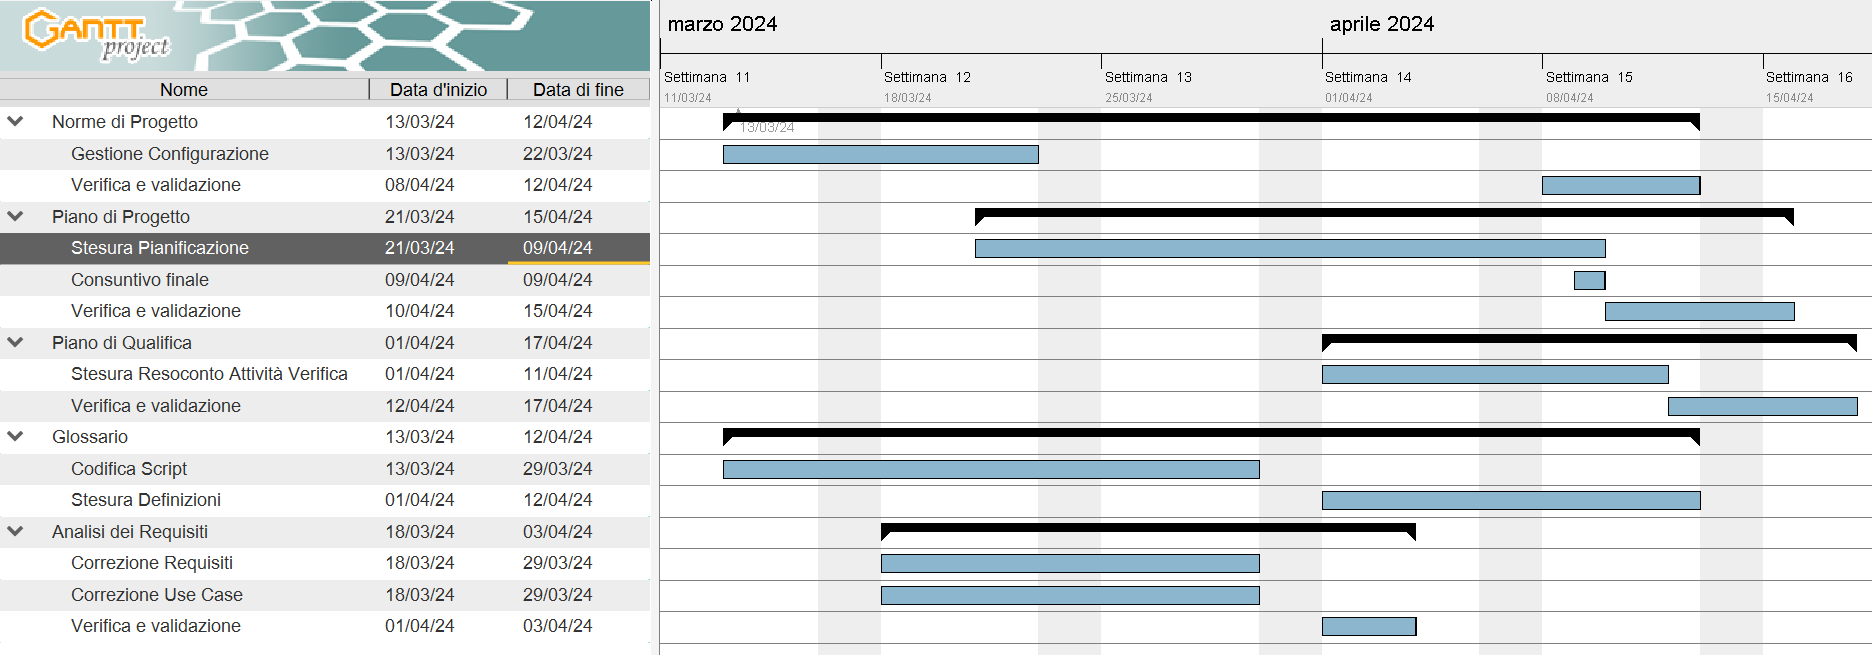
\includegraphics[scale=.5]{GanttQuartoPeriodo.png} \end{figure}

\textbf{Consuntivo orario}

\begin{tblr}{
    colspec={|X[5cm]|X[.5cm]|X[.5cm]|X[.5cm]|X[.5cm]|X[.5cm]|X[.5cm]|X[3.5cm]},
    row{odd}={bg=white},
    row{even}={bg=lightgray},
    row{1}={bg=black, fg=white},
    row{8}={bg=black, fg=white}
}

    Nominativo & Re & Am & An & Pg & Pr & Vf & Ore Totali \\ \hline
    Alberto C. & - & - & - & 2 & - & 3 & 5 \\ \hline
    Bilal El M. & 2 & - & 4 & 2 & - & 5 & 13 \\ \hline
    Alberto M. & - & - & 4 & - & - & 5 & 9 \\ \hline
    Alex S. & 5 & 5 & - & - & - & - & 10 \\ \hline
    Iulius S. & - & - & 4 & - & - & 5 & 9 \\ \hline
    Giovanni Z. & - & - & - & 5 & - & 5 & 10 \\ \hline
    Totale & 7 & 5 & 12 & 9 & - & 23 & 56 \\ \hline

\end{tblr}

\textbf{Consuntivo economico}

\begin{tblr}{
colspec={|X[5cm]|X[3.5cm]|X[1.5cm]|X[3.5cm]},
row{odd}={bg=white},
row{even}={bg=lightgray},
row{1}={bg=black, fg=white},
row{8}={bg=black, fg=white}
}

Ruolo & Costo orario (€/h) & N. Ore & Costo totale (€) \\ \hline
Responsabile & 30,00 & 7 & 210,00 \\ \hline
Amministratore & 20,00 & 5 & 100,00 \\ \hline
Analista & 25,00 & 12 & 300,00 \\ \hline
Progettista & 25,00 & 9 & 225,00 \\ \hline
Programmatore & 15,00 & 0 & 0,00 \\ \hline
Verificatore & 15,00 & 23 & 345,00 \\ \hline
Totale & \SetCell[c=1]{c} & 56 & 1.180,00 \\ \hline

\end{tblr}

\textbf{Gestione dei ruoli}

\paragraph{}
Come si può vedere dalla suddetta tabella, in questo quarto periodo il gruppo ha concentrato buona parte del monte-ore nello svolgimento
del ruolo di Analista e soprattutto di Verificatore: Per quanto concerne il primo, i membri hanno speso il 21\% delle risorse al fine di completare la stesura di tutta la documentazione e di effettuare le correzioni all'Analisi dei Requisiti
in seguito alla revisione del prof. Cardin; in previsione della seconda fase della RTB, una parte cospicua di risorse (\%50) è stata utilizzata per la fase di verifica
e validazione della documentazione sopracitata; il gruppo ha inoltre riservato il 12\% delle ore al ruolo del Responsabile, data l'importanza di un efficace
ed efficiente orchestrazione delle attività del gruppo in vista della seconda parte della RTB, e il 9\% di ore alla figura dell'Amministratore, al fine
di evitare potenziali conflitti negli item di versionamento prodotti dai differenti membri; infine, il 16\% delle risorse è stato dedicato al Progettista.

\paragraph{Gestione dei rischi}

\begin{itemize}
    \item \textbf{Rischio verificatosi:} Conflitti decisionali:
    \begin{itemize}
        \item \textbf{Esito Piano di Contingenza:} In seguito alla revisione della Technology Baseline effettuate dal prof. Cardin, sono emerse criticità nella progettazione del PoC e in particolare nella scelta dello stack tecnologico; è stata quindi avviata una discussione tra i membri del gruppo su come risolvere tali criticità, consci della tabella di marcia da seguire rigorosamente al fine di completare la revisione PB evitando ulteriore ritardo a quello già accumulato. Data la natura sensibile dell'oggetto della discussione, i membri hanno faticato più del previsto a trovare una soluzione condivisa da tutti;
        \item \textbf{Impatto:} L'impatto dei conflitti decisionali riguardanti eventuali modifiche dello stack tecnologico non è ancora misurabile, poiché non è prevedibile allo stato attuale se avverrà una modifica dello stack, e in caso quest'ultima avvenga, una misura quantitativa delle risorse che il gruppo dovrà forzatamente riallocare.
    \end{itemize}
\end{itemize}

\textbf{Retrospettiva:} \\
Come si evince dalla tabella del consuntivo orario, in questo quarto periodo il gruppo si è prodigato nel terminare la stesura di tutta la documentazione restante,
e nelle successive operazioni di verifica e validazione; in seguito alla revisione TB effettuata dal prof. Cardin, sono state apportate le necessario modifiche all'Analisi
dei Requisiti.\\
Inoltre, a seguito delle perplessità espresse dal prof. Cardin riguardo le scelte riguardo lo stack tecnologico, il gruppo si è visto costretto a dedicare parte delle risorse ad
un nuovo lavoro di studio e ricerca per capire se includere nuovi framework o linguaggi nello stack tecnologico, soprattutto in previsione della progettazione dell'MVP.
\begin{itemize}
    \item \textbf{Obbiettivi raggiunti:}
    \begin{itemize}
        \item Stesura della prima versione delle Norme di Progetto;
        \item Stesura della prima versione del Piano di Progetto;
        \item Stesura della prima versione del Piano di Qualifica;
        \item Creazione di uno script per l'individuazione di tutti i termini facenti parte del Glossario;
        \item Stesura della prima versione del Glossario;
        \item Candidatura per la seconda parte dell'RTB;
        \item Stesura della seconda versione dell'Analisi dei Requisiti.
    \end{itemize}
    \item \textbf{Obiettivi mancati:}
    \begin{itemize}
        \item Nessuno.
    \end{itemize}
\end{itemize}